\documentclass{article}

\setlength{\parindent}{0pt}

\usepackage{fullpage}
\usepackage{graphicx}

\def\Nat{{\rm I\kern-.17em N}}
\def\SFF{\hbox{I\kern-.09em\hbox{I}}}
\newcommand\Bezier{B\'{e}zier }

\newcommand\projecttitle{Windy Awakening}
\newcommand\myname{Kevin Haslett}
\newcommand\myuserid{kahaslet}
\newcommand\mystudentid{20468033}

\begin{document}

\begin{minipage}[t]{3in}
{\huge \bf 
	\projecttitle 
}

\medskip
Name: \myname \\ 
User ID: \myuserid \\ 
Student ID: \mystudentid 
\end{minipage}
\hfill
\begin{minipage}[t]{3in}
%%%% Use the first of these if your image is wider than tall; use the
%%%% second if your image is taller than it is wide.
\vspace{0pt}
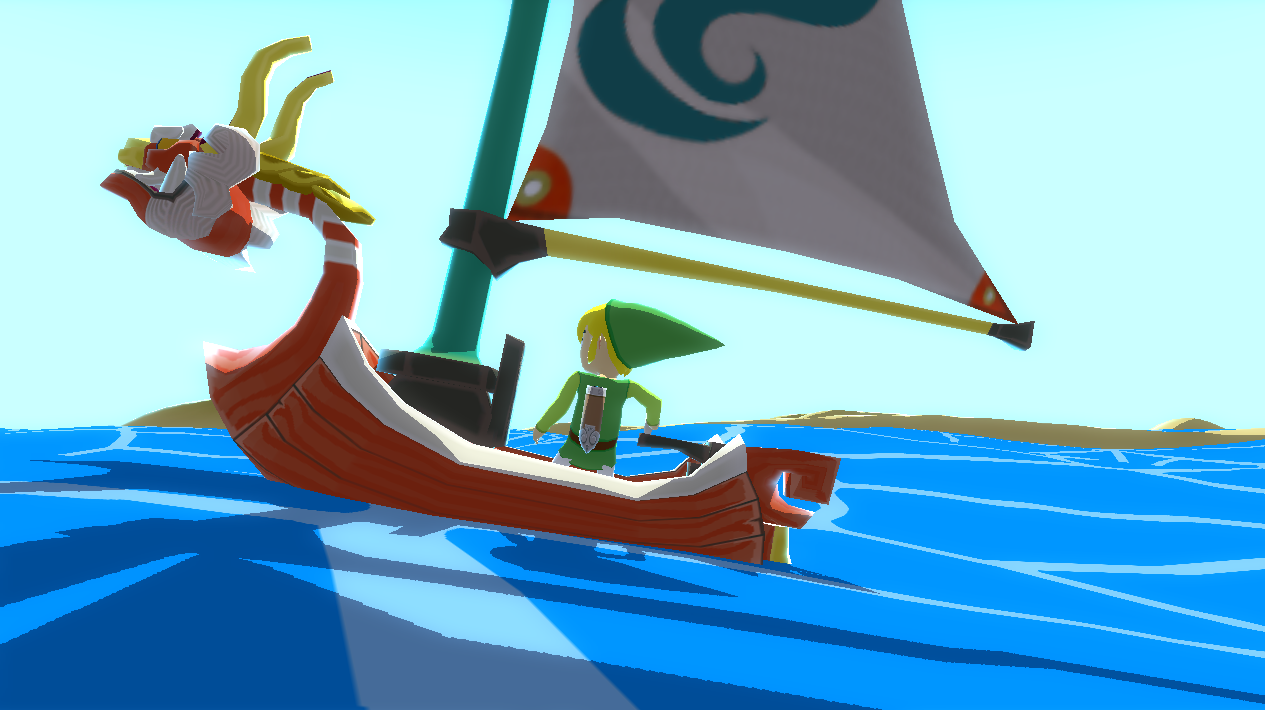
\includegraphics[width=3in]{screenshot1.png}   %%%% Change file.png to your image
% \includegraphics[height=2in]{image2-FRONT.png}   %%%% Change file.png to your image
\end{minipage}


\subsection*{Artistic Merit (Polish/Artistry/Humour)}
\vfill
\subsection*{Technical Merit (Algorithms/User Interface/Graphics Techniques)}
\vfill
\subsection*{Difficulty}
\vfill
\subsection*{Code/Documentation/Demo}
\vfill
\subsection*{Mark}
\begin{center}
\begin{tabular}{lr}
Objective Mark: &~~/10\\
Subjective Mark: &~~/6\\
\hline
Total &~~/16
\end{tabular}
\end{center}

\newpage

{\huge \bf 
	\projecttitle 
}

\medskip
Name: \myname \\ 
User ID: \myuserid \\ 
Student ID: \mystudentid 

\bigskip
{\Large Objectives}

\hrule
\begin{description}
        \item[\_\_\_ 1:]
          Texture Mapping

        \item[\_\_\_ 2:]
		  Cell Shading

        \item[\_\_\_ 3:]
		  Shadow Mapping
			
        \item[\_\_\_ 4:]
		  Bloom Shader

        \item[\_\_\_ 5:]
		  Gooch Lighting Model and Day/Night Cycle

        \item[\_\_\_ 6:]
	      Voronoi Diagrams

        \item[\_\_\_ 7:]
		  Edge Detection

        \item[\_\_\_ 8:]
		  Gaussian Blur and Threshold Mapping to Generate Final Water Texture

        \item[\_\_\_ 9:]
		  Island Terrain Generated Using Perlin Noise

        \item[\_\_\_ 10:]
		  Simple Sailing Physics\\

		{\Large Extra Objectives}		    
		\hrule
		  
        \item[\_\_\_ 11:]
		  Animated Infinite Water Geometry
		  
        \item[\_\_\_ 12:]
		  Gradient Texture Sampling and Beautiful Sunset
		  
        \item[\_\_\_ 13:]
		  Rigging and Posing Models

\end{description}

\hrule

\end{document}
